	\begin{figure}[H]
		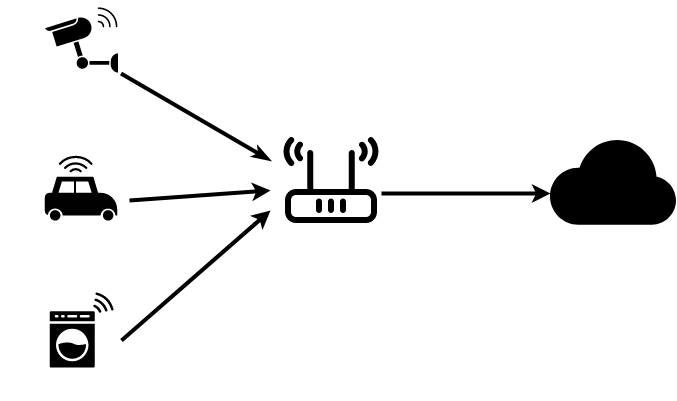
\includegraphics[scale=0.4]{typical_iot_arch.png}		
		\centering	
		\caption{Example of an IoT architecture \cite{iot-example-icons}.}
		\label{fig:iotArchExample}
	\end{figure}	
	A simplified \ac{IoT} system architecture that is most commonly found in the production installations contains of three parts - IoT Nodes, IoT Gateways, and Cloud Services (figure \ref{fig:iotArchExample}).\\
	IoT Nodes are small \ac{IoT} devices such as light sensors, temperature sensors, actuators, and others. 
		They connect to the \ac{IoT} Gateway through various wireless and cable protocols and send measurements.\\
		In a real-life installation case there can be thousands of devices connecting to a gateway. \\
		IoT Gateway is a "proxy" between the Cloud and the IoT Nodes.
		The nodes connect to it through a range of protocols and send measurements. 
		The gateway usually takes care of authentication and authorization.
		It collects the measurements, aggregates them, and sends to the cloud.\\
		Cloud Services are services running on remote servers.
		It is usually a distributed setup, capable of storing and processing extremely large amounts of data.
		The Cloud Services receive measurements from IoT Gateways, process them, and eventually persist.